\section{Metodologia}

O presente projeto apresenta o desenvolvimento de um sistema \gls{cad}, a partir de uma arquitetura de \textit{visual transformers}, em que desse modelo terá a tarefa de lidar com a base de dados de imagens que foi fornecida pela \gls{fmabc}, sendo essa base composta de imagens de pacientes brasileiros afetados pela psoríase e pacientes com dermatite. A intenção dessa proposta é que a combinação de diferentes análises e informações traga um aumento na precisão desse tipo de sistema, fornecendo um suporte à tomada de decisão. Efetivamente, será implementada uma solução de ponta a ponta, que exigirá desde técnicas para o tratamento e preparo dos dados, até soluções para o refinamento do modelo de \gls{ia}.

A partir dos conceitos de redes neurais artificiais e \textit{transformers}, fica mais claro entender a construção dos modelos de \gls{ia}, que seguem um certo fluxo padrão, esse fluxo é conhecido como \textit{pipeline}. Os \textit{pipelines} de \gls{ia} envolvem todo o fluxo de atividades necessárias para o funcionamento apropriado do modelo. De modo genérico, este fluxo geralmente começa com atividades relacionadas à extração, transformação e carregamento dos dados, processo conhecido como \gls{etl}; no caso de modelos de \gls{ia} voltados a visão computacional, essa fase utiliza técnicas para preparar essas imagens a um modelo de \gls{ia}, geralmente envolvendo atividades relacionadas ao processamento digital de imagens. Além das transformações nas imagens é necessário realizar uma estratificação dos dados, uma parte deve ser separada para o treinamento da rede, enquanto a outra deve ser exclusivamente voltada para a validação da rede. A etapa seguinte envolve o treinamento da rede, essa etapa exige diferentes técnicas para o sucesso do modelo, entre essas técnicas estão a escolha de um algoritmo de otimização adequado ao problema, o uso de uma função de perda apropriada, ajuste correto dos hiperparâmetros da rede e número de épocas no treinamento. As subseções a seguir destacam cada uma das fases do pipeline aplicado para o desenvolvimento do modelo.

\subsection{Coleta de dados}

A etapa de coleta de dados configura-se da responsabilidade de estabelcer formas consistentes de acesso aos dados, também deve garantir segurança e a integridade dessas informações. Para a realização da coleta de dados, foram desenvolvidos \textit{scripts} utilizando a linguagem de programação Go, uma ferramenta que ganhou muita popularidade devido a sua performance. O desenvolvimento desses \textit{scripts} permitiram que todo o manuseio das informações fosse realizado de forma automatizada, além de coletar os dados, também envolvem tarefas como catalogação das informações.


\begin{figure}[h] % Ajuste largura
    \centering
    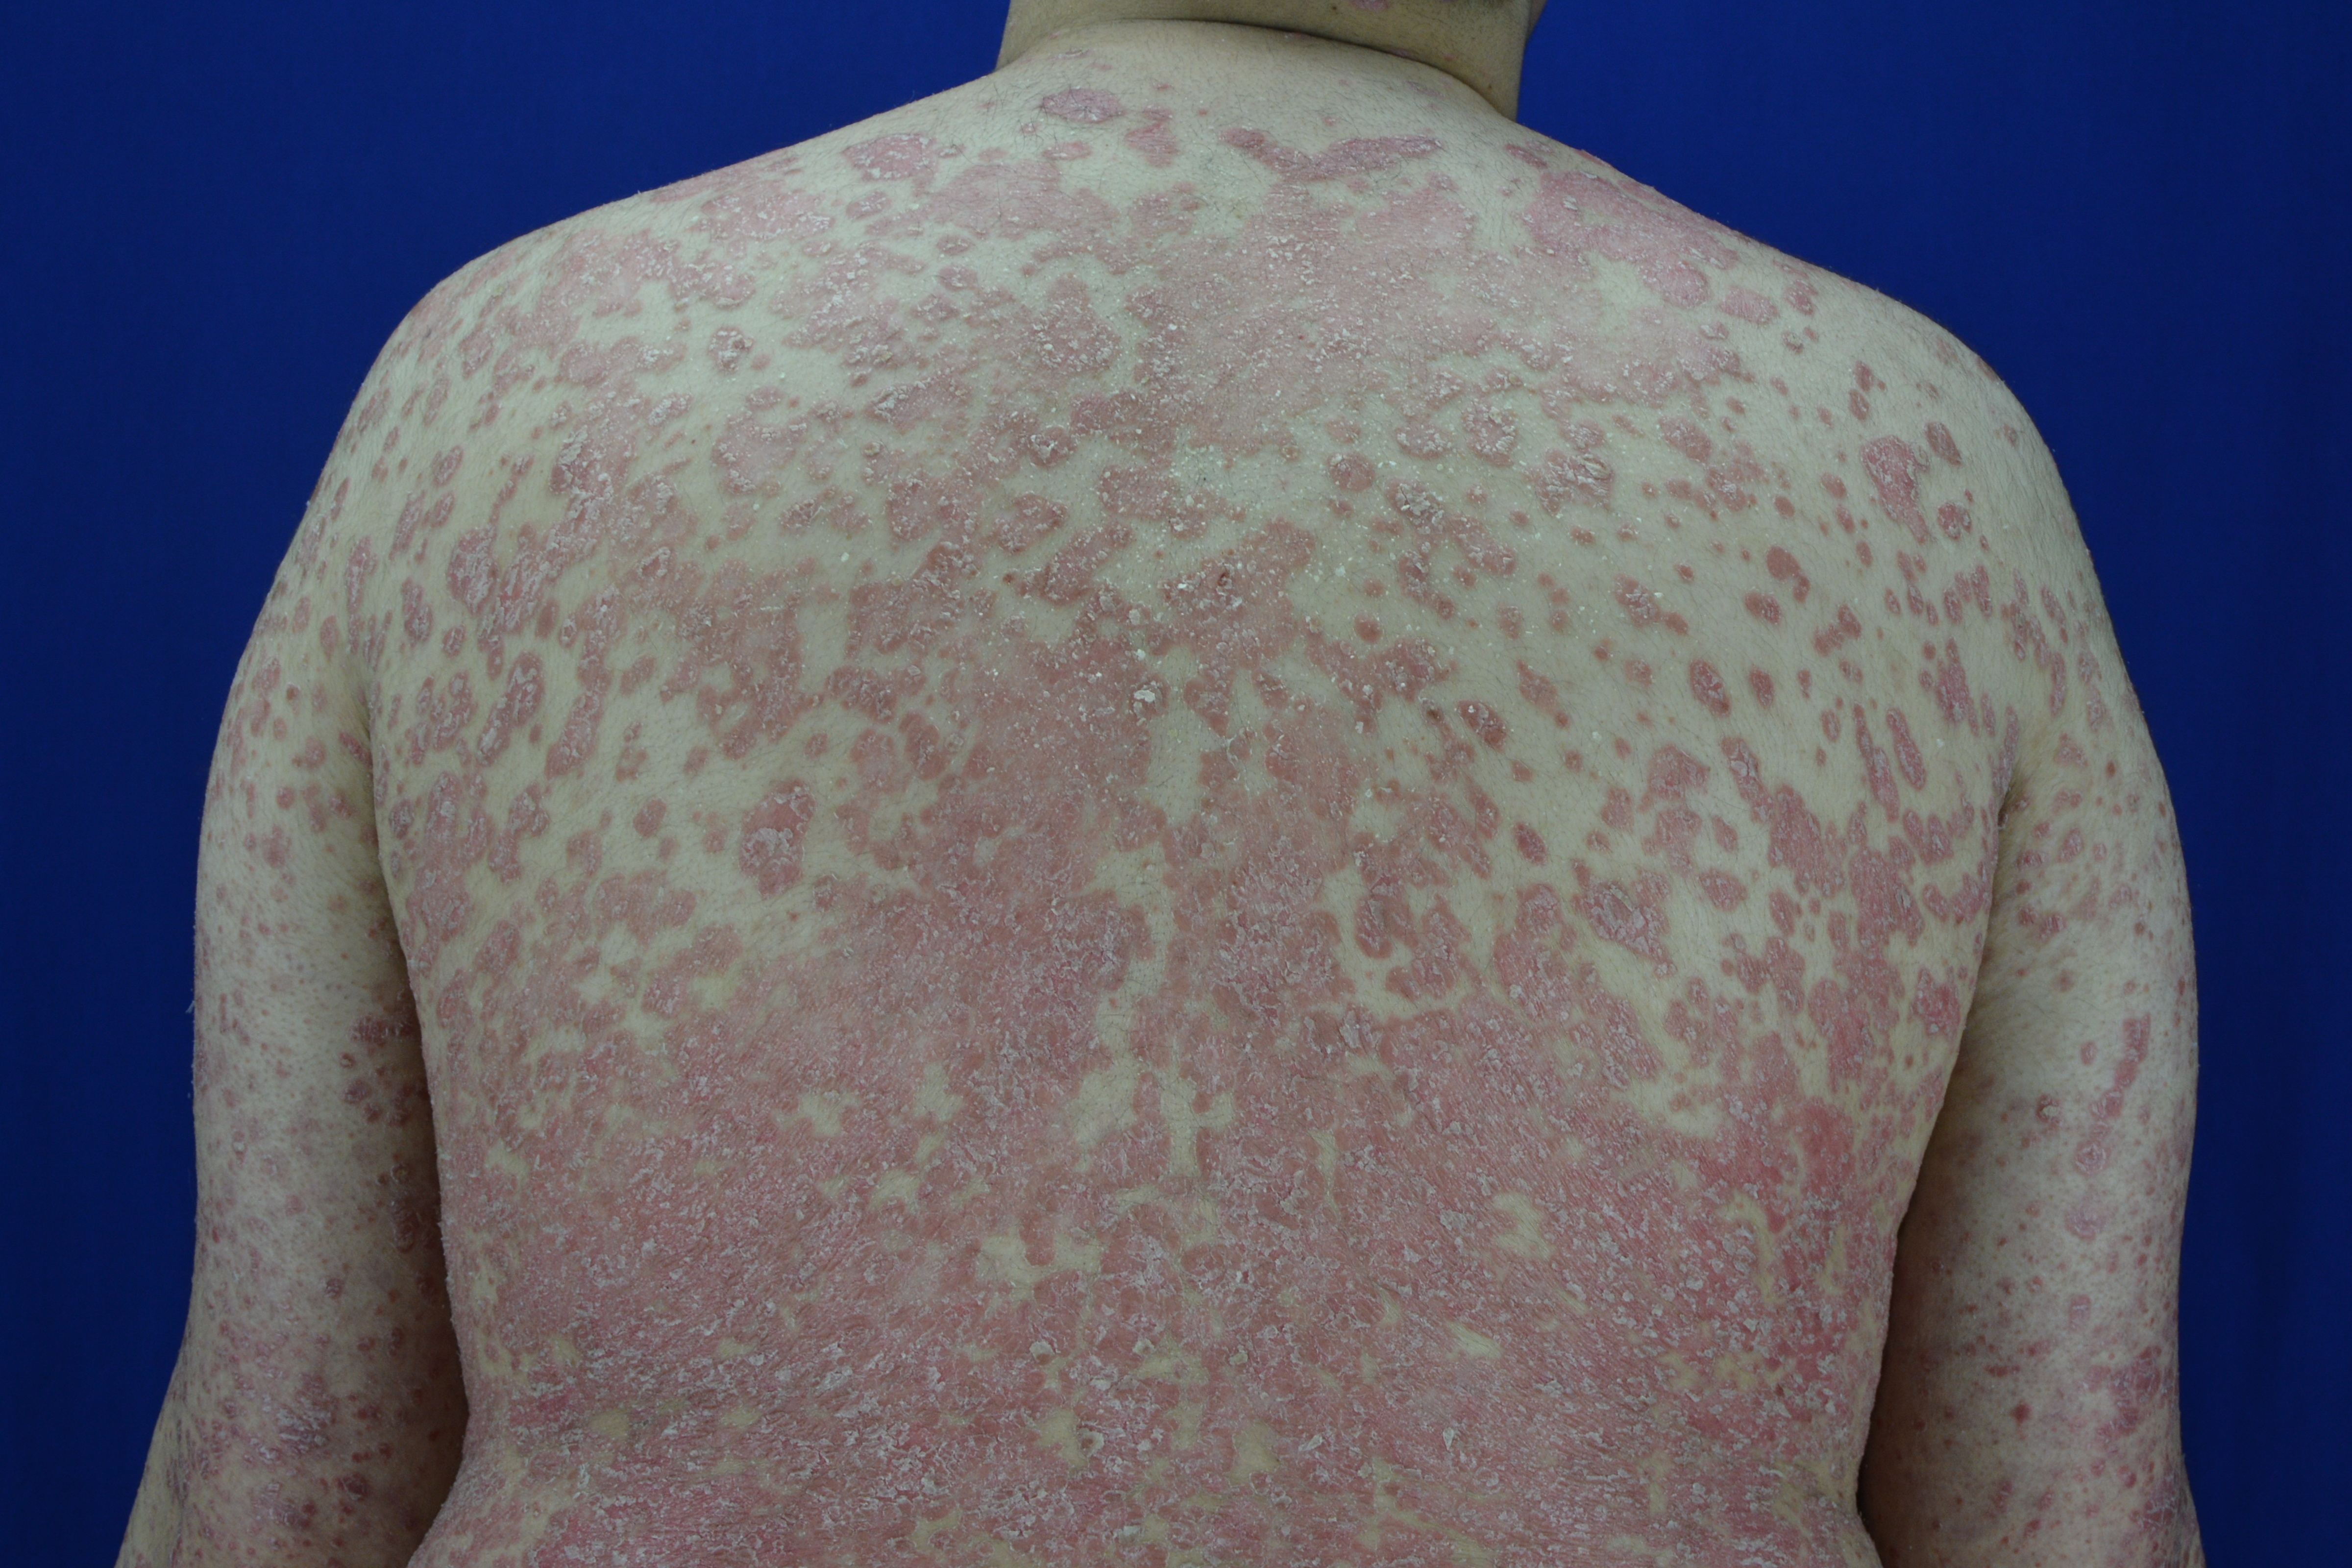
\includegraphics[width=0.6\textwidth]{images/dataset_example.jpg}
    \caption{Imagem de paciente com psoríase (FMABC, 2025)}
    \label{fig:ex-dataset}
\end{figure}

\subsubsection{Pré processamento}

Durante essa fase, foram estudadas quais seriam as técnicas aplicadas para preparar os dados coletados ao modelo. Nessa fase foram encontrados alguns desafios, entre eles o primeiro é a limitação no número de amostragens recebidas pela instituição parceira e desbalanceamento entre as classes de dados, ou seja, na prática haviam muito mais imagens da categoria psoríase.

Antes do uso desses dados para o modelo, foi necessário uma inspeção manual sobre o dataset, que resultou na exclusão de muitas imagens, devido a fatores como baixa qualidade, por exemplo imagens que estavam muito embaçadas ou com baixa resolução, e representação inadequada da classe, em que algumas fotografias que mostravam o corpo todo, e não a área lesionada. A utilização de tais imagens poderiam introduzir ruído e prejudicar a capacidade de generalização do modelo. Adicionalmente, foi executado um pré-processamento específico para remover o fundo azul comum na maioria das imagens, assegurando que o modelo focasse exclusivamente nas características morfológicas das lesões.

Para lidar com as limitações mencionadas anteriormente, foram desenvolvidos e aplicados algoritmos de \textit{image augmentation}, esses algoritmos operam da seguinte maneira, iteram sobre os dados fornecidos, e a partir destes, geram novos dados com filtros pré determinados. Nessa aplicação, os filtros utilizados foram de \textit{random cropping}, que aplica um corte numa posição aleatória da imagem, com essa técnica.

Outro desafio encontrado durante o pré processamento foram as dimensões das imagens, já que as imagens tinham dimensões por volta de 2400x3800 pixels, e esse tipo de arquitetura trabalha com entradas de 521x521 pixes, assim todas as tentativas de aplicar redimensionamento nas imagens não tiveram bons resultados, pois houve uma perda muito grande de qualidade dos dados, a alternativa encontrada para lidar com isso foi o uso já mencionado de \textit{random cropping}, pois o cropping descarta a necessidade de alterar os pixels da imagem, apenas usar um recorte de uma área randomica.


\begin{figure}[h] % Ajuste largura
    \centering
    \includegraphics[width=0.5\textwidth]{images/pre_processamento_psoriasis_jitter.png}
    \caption{Imagem de paciente com psoríase (CORRÊA, 2025)}
    \label{fig:ex-dataset}
\end{figure}
No processo de \textit{data augmentation}, também foi aplicado a rotação das imagens na horizontal e vertical, assim a mesma amostra porém em posição diferente poderia ser utilizada para treinamento da rede, o que enriqueceu o dataset e fortaleceu a capacidade de generalização do modelo. 
Além do aumento da base de dados, foram aplicadas transformações no domínio de cores das imagens. As imagens foram convertidas para o domínio de cor YCbCr, muitos \textit{softwares} de edição de imagens utilizam esse domínio para manipulação desses dados. A principal vantagem desse domínio é a separação da informação de luminância (canal Y) da informação de crominância (canais Cb e Cr)

Por fim, todas as imagens foram normalizadas, um passo crucial para o treinamento de redes neurais. O procedimento de normalização consistiu em ajustar os valores dos pixels para o intervalo [0, 1], o que garante que a rede não seja afetada pela escala dos dados de entrada, promovendo uma convergência mais rápida e estável do modelo.

\subsection{Treinamento do modelo}

Para avaliar o desempenho do modelo de forma robusta e imparcial, foi utilizada a validação cruzada com \textit{k-folds} estratificada. O conjunto de dados foi dividido em \(k= [Número de folds]\) \textit{folds}, garantindo que a proporção das classes fosse mantida em cada partição de treinamento e teste. Essa abordagem minimizou a dependência do modelo em relação a uma única divisão de dados.

A partir de um processo exploratório, em que foram aplicados diferentes testes com modelos de \gls{cnn} e \textit{Visual Transformers}, para identificar a configuração mais adequada para a tarefa de classificação binária de doenças de pele. As arquiteturas investigadas incluíram modelos de redes neurais convolucionais (\gls{cnn}), como VGG16 e ResNet152, e arquiteturas baseadas em transformadores, como Visual Transformers (\textit{ViT}) e Swin Transformers. Após uma análise comparativa, a arquitetura \textit{Swin Transformers} foi selecionada para o modelo final.

De modo a otimizar a busca por hiperparametros ideais para o objetivo proposto, foi utilizado uma técnica de \textit{Grid Search}, que consiste em testar e avaliar o desempenho de todas as combinações de parâmetros previamente fornecidos de forma automática. A Tabela \ref{tab:hiperparametros} apresenta os valores finais selecionados após a aplicação desta técnica.

\begin{table}[h]
    \centering
    \label{tab:hiperparametros}
    \begin{tabular}{ll}
        \toprule
        \textbf{Hiperparâmetro} & \textbf{Valor} \\
        \midrule
        Otimizador              & SGD (\textit{Stochastic Gradient Descent}) \\
        Taxa de aprendizado     & 0.01 \\
        Momento (\textit{Momentum})     & 0.9 \\
        Decaimento de peso      & 0.001 \\
        Função de perda         & Entropia Cruzada Binária (\texttt{BCELoss}) \\
        Tamanho do lote         & 32 \\
        Número de épocas        & 40 \\
        Scheduler               & \texttt{ReduceLROnPlateau} \\
        \bottomrule
    \end{tabular}
    \caption{Hiperparâmetros finais utilizados no treinamento do modelo.}
\end{table}


\subsection{Análise e discussao dos resultados}

A avaliação do modelo incluiu análise quantitativa e qualitativa para compreender sua capacidade de tomada de decisão. Para tal, foram empregadas duas abordagens complementares: a análise de métricas de desempenho estatísticas e a interpretação visual por meio de mapas de calor.

A performance do modelo foi mensurada utilizando métricas de classificação padrão para problemas binários.Conforme os resultados desses métodos, foi possível analisar se o desempenho do modelo está de acordo com o esperado. Dentre as técnicas mais comuns, foram utilizadas métricas como acurácia, definida pela fórmula 

\begin{equation}
  acurácia = \frac{VP +VN}{VP + FN + VN + FP} \; ,
    \label{eq: acuracia}
\end{equation}

em que \(VP\) é a quantidade de verdadeiros positivos; \(VN\) é a quantidade de verdadeiros negativos; \(FN\) é a quantidade de falsos negativos e \(FP\) é a quantidade de falsos positivos. Em seguida, a métrica de precisão foi utilizada, determinada pela fórmula:

\begin{equation} 
  precisão = \frac{VP}{VP + VN} \; ,
  \label{eq: precisao}
\end{equation}

E por último, uma métrica de avaliação chamada sensibilidade, estabelecida pela fórmula:

\begin{equation}
sensibilidade = \frac{VP}{VP + FN} \; ,
  \label{eq: sensibilidade}
\end{equation}

Também foi empregada a **revocação** (\textit{recall}), uma métrica que mede a capacidade do modelo de encontrar todas as amostras positivas, estabelecida pela fórmula:

\begin{equation}
revocação = \frac{VP}{VP + FN}
  \label{eq:revocacao}
\end{equation}

Por fim, o \textit{F1-Score}, que representa a média harmônica entre precisão e revocação, foi utilizado como uma métrica de equilíbrio para avaliar o modelo em cenários com classes desbalanceadas.

\begin{equation}
  F1 = 2 \cdot \frac{Precisão \cdot Revocação}{Precisão + Revocação}
  \label{eq:f1_score}
\end{equation}

Para estabelecer os mapas de calor e promover uma compreensão visual dos resultados do modelo, a ferramenta utilizada para essa tarefa é foi o \textit{GradCam}, uma ferramenta de interpretabilidade que gera mapas de calor para qualquer camada convolucional de uma rede neural. Esses mapas destacam as regiões da imagem de entrada que mais influenciaram a decisão do modelo para uma determinada classe.


\begin{figure}[h]
  \begin{center}
    \includegraphics[scale=0.4]{images/test1-compesos.png}
  \end{center}
  \caption{Resultado da classificacão do modelo com \textit{GradCam}}
  \label{fig:gradcam}
\end{figure}


Na Figura \ref{fig:gradcam}, é apresentado um exemplo de um mapa de calor gerado pelo Grad-CAM para a classe Psoríase. A análise da imagem demonstra que as regiões de maior ativação da rede (indicadas pelas cores quentes, como amarelo e vermelho) correspondem diretamente à área da lesão dermatológica. Essa observação valida o comportamento do modelo, confirmando que ele não se baseia em ruídos ou em informações de fundo, mas sim nas características morfológicas da lesão, que são clinicamente relevantes para o diagnóstico.


% % --- Poderia ficar nos objetivos? ---
% % Além do desenvolvimento de um modelo que seja capaz de segmentar imagens microscópicas de células com alta precisão, esse trabalho também propõe a aplicação desse modelo num sistema destinado a uso médico. 

